The XML benchmarking project XMARK~\cite{xmark/original} is one of the most popular and most commonly used XML benchmarking project to date. It provides a small executable tool called \textit{xmlgen} that allows for the creation of a synthetic XML dataset based on a fixed schema describing an Internet auctions database. Its generator can be used to build  a single record with a large, hierarchic XML tree structure. A factor can be specified to scale the generated data, ranging from a few kilobytes to any arbitrary size limited by the capacity of the system. The textual part of resulting XML document is constructed from 17,000 most frequently occurring words of Shakespeare's plays.
\label{xmark-dataset}
\subsubsection{Dataset}
The main entities of XMark data come with two group. In first group \texttt{person},\texttt{open\_auction}, \texttt{closed\_auction}, \texttt{item} and \texttt{category} are expressed through the reference as in Fig.~\ref{fig:xmark-reference} whereas second group entities \texttt{annotation} and \texttt{description} take after the natural language text and are document-centric element structure. \texttt{annotation} and \texttt{description} are embedded into sub-tree of group one entities. 
\\
As shown in Fig.~\ref{fig:xmark-tree}, \texttt{items} are the objects for sale or already sold. Each \texttt{item} caries a unique identifier and having properties like payment information(credit card, money order), \texttt{description} , a reference to the seller etc., all encoded as element. Each item is assign to world region like \texttt{asia}, \texttt{africa} etc. as a parent of an item. \texttt{open\_auctions} are auctions in progress which contains bid history(increase/decrease over time) with reference to bidder and seller, current bid etc. \texttt{closed\_auctions} are the auctions that are completed, which has reference to buyer, seller and item that is sold, amount of price etc. \texttt{people} are the information about \texttt{person} that are connected to buyer/seller of open\_auctions, closed\_auctions etc. \texttt{categories} are implemented to classify items which has a name and description. A \texttt{catgraph} links categories into a network.  The full semantic of XMark dataset can be found in~\cite{xmark/original}.
	%\tikzset{
	basic/.style  = {draw, text width=2cm, drop shadow, font=\sffamily, rectangle},
	root/.style   = {basic, rounded corners=2pt, thin, align=center,
		fill=green!30},
	level 2/.style = {basic, rounded corners=6pt, thin,align=center, fill=green!60,
		text width=8em},
	level 3/.style = {basic, thin, align=left, fill=pink!60, text width=6.5em}
}
\begin{tikzpicture}[
level 1/.style={sibling distance=40mm},
edge from parent/.style={->,draw},
>=latex]

% root of the the initial tree, level 1
\node[root] {Drawing diagrams}
% The first level, as children of the initial tree
child {node[level 2] (c1) {Defining node and arrow styles}}
child {node[level 2] (c2) {Positioning the nodes}}
child {node[level 2] (c3) {Drawing arrows between nodes}};

% The second level, relatively positioned nodes
\begin{scope}[every node/.style={level 3}]
\node [below of = c1, xshift=15pt] (c11) {Setting shape};
\node [below of = c11] (c12) {Choosing color};
\node [below of = c12] (c13) {Adding shading};

\node [below of = c2, xshift=15pt] (c21) {Using a Matrix};
\node [below of = c21] (c22) {Relatively};
\node [below of = c22] (c23) {Absolutely};
\node [below of = c23] (c24) {Using overlays};

\node [below of = c3, xshift=15pt] (c31) {Default arrows};
\node [below of = c31] (c32) {Arrow library};
\node [below of = c32] (c33) {Resizing tips};
\node [below of = c33] (c34) {Shortening};
\node [below of = c34] (c35) {Bending};
\end{scope}

% lines from each level 1 node to every one of its "children"
\foreach \value in {1,2,3}
\draw[->] (c1.195) |- (c1\value.west);

\foreach \value in {1,...,4}
\draw[->] (c2.195) |- (c2\value.west);

\foreach \value in {1,...,5}
\draw[->] (c3.195) |- (c3\value.west);
\end{tikzpicture}
	

\begin{figure}
	\centering
	\subfigure[Reference in \textit{XMark}]{
		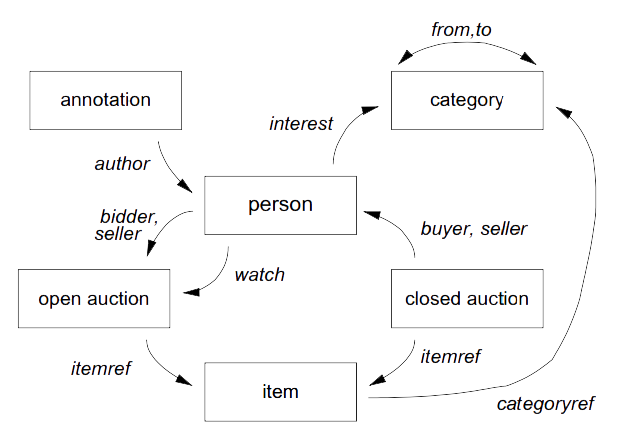
\includegraphics[width=0.40\textwidth]{img/xmark-references.png}{
			\label{fig:xmark-reference}
		}
	}
	\centering
	\subfigure[Reference in \textit{XMark} dataset tree~\cite{xmark/original}]{
		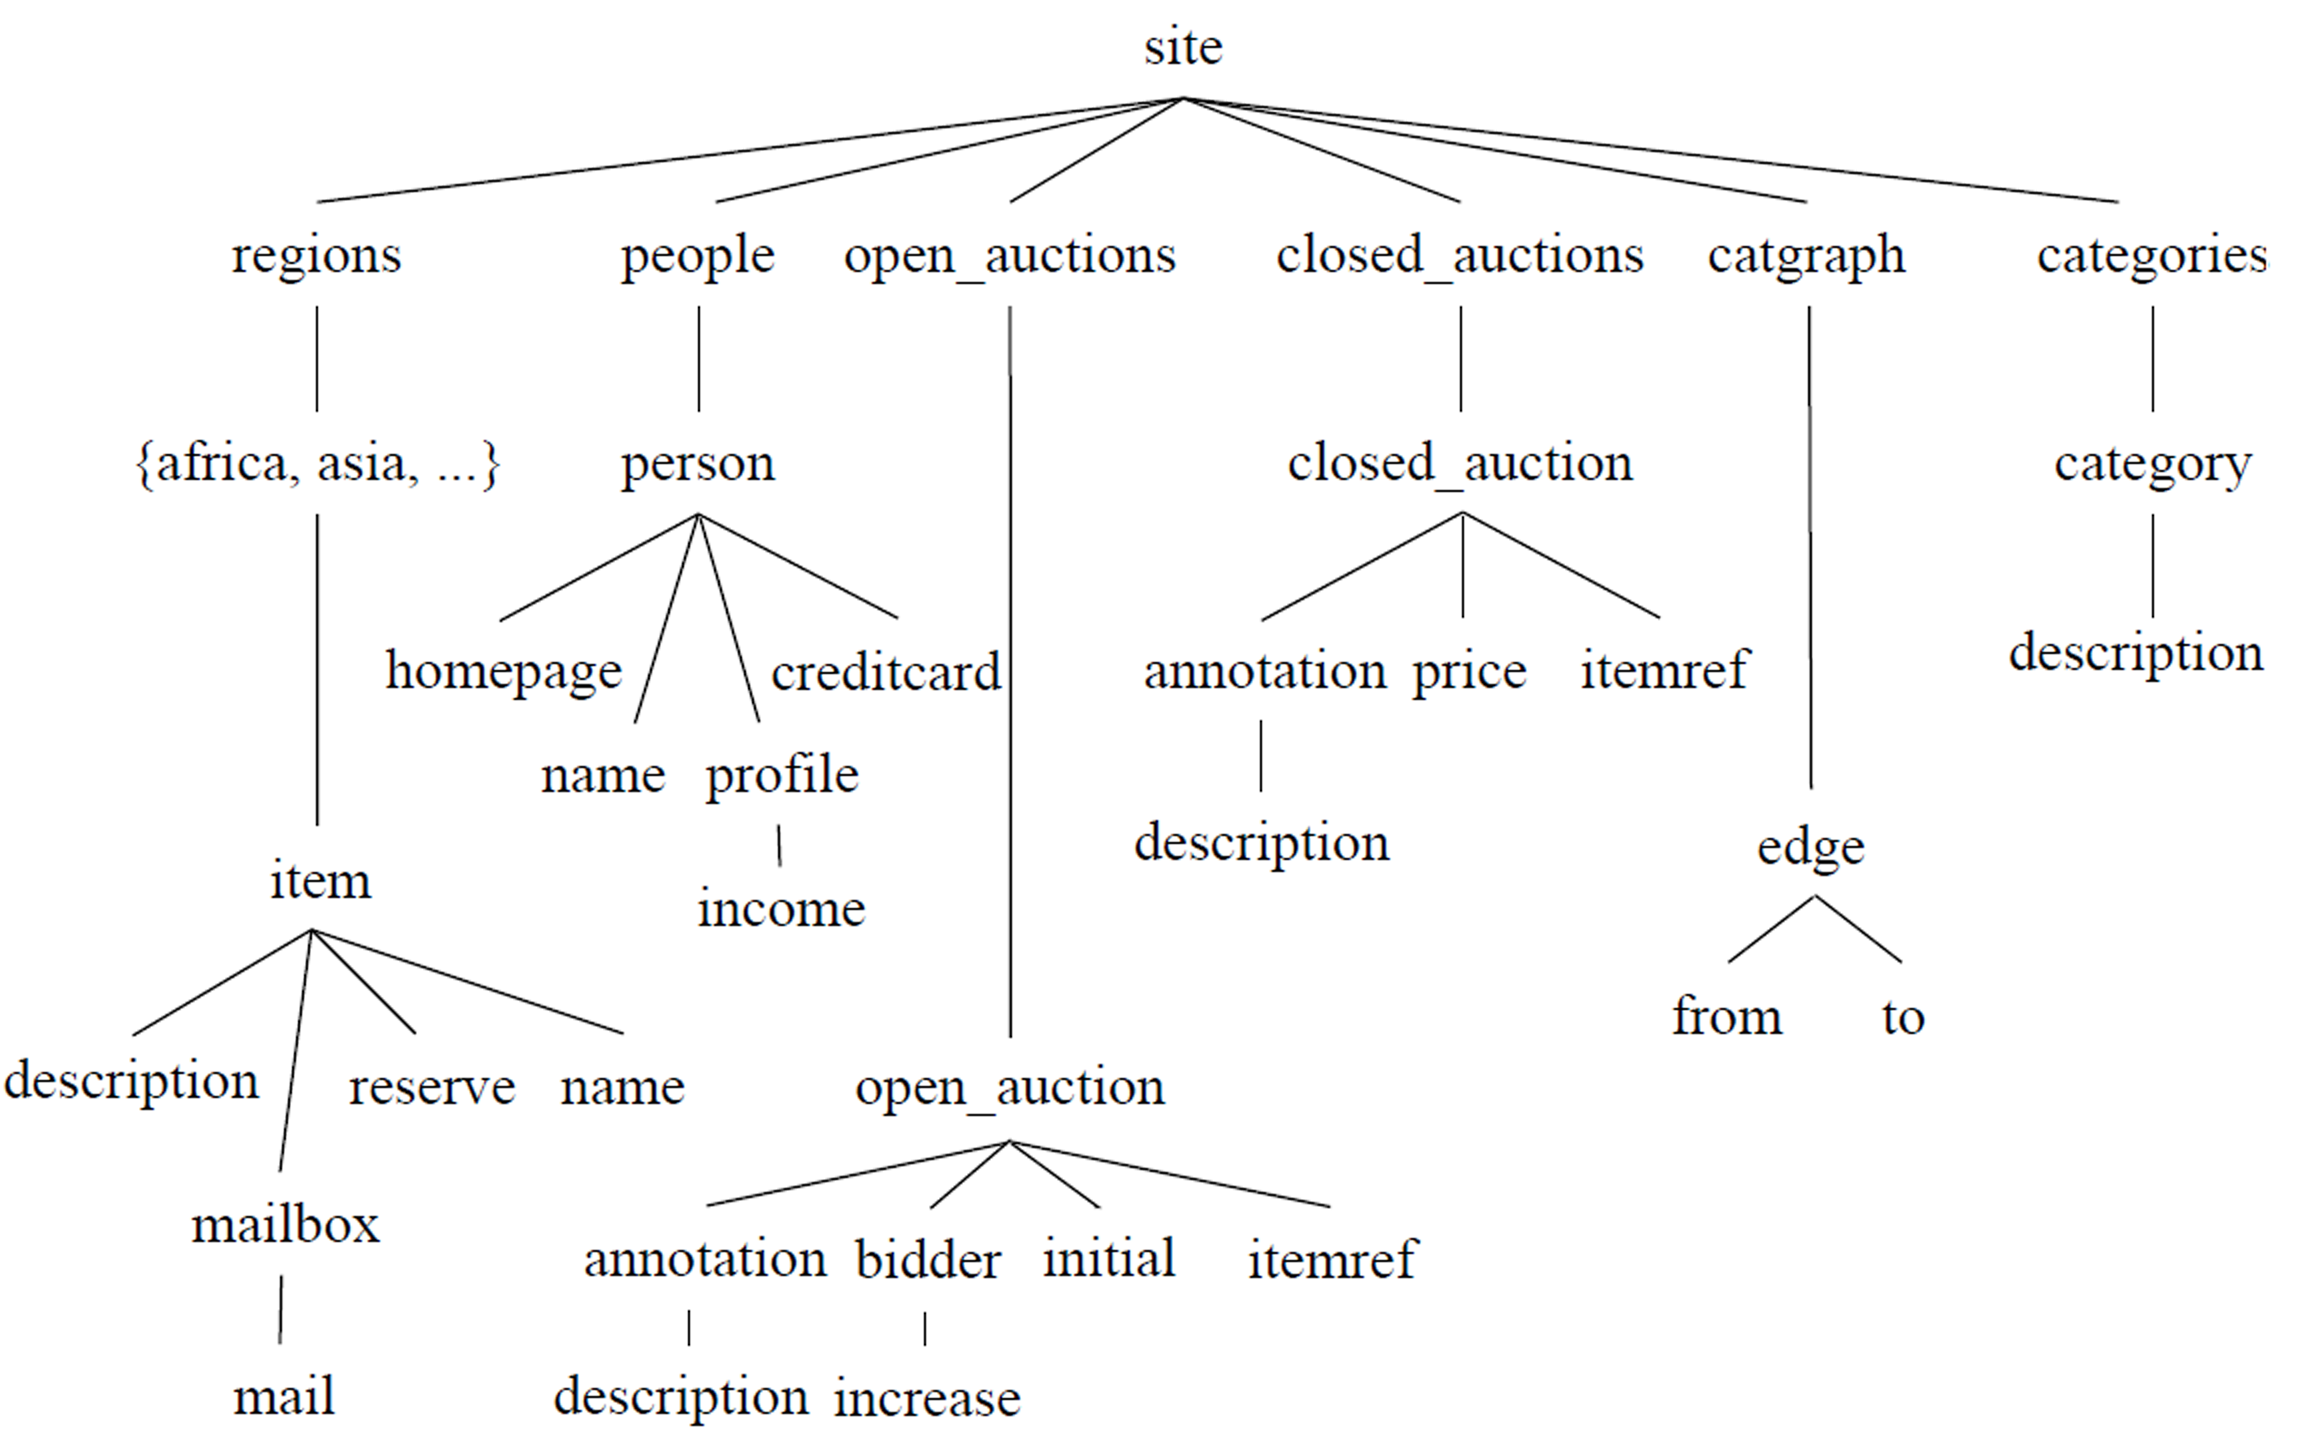
\includegraphics[width=0.40\textwidth]{img/xmark-tree.png}{
			\label{fig:xmark-tree}
		}
	}
	\caption{XMark data tree and reference}
	\label{fig:xmark-tree-reference}
\end{figure}
\begin{figure}
	\centering
	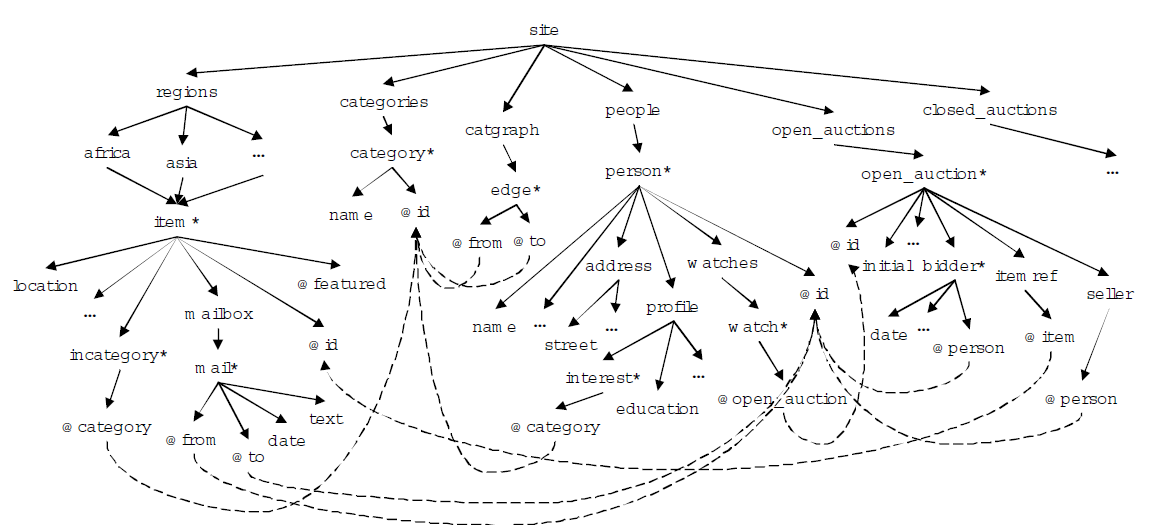
\includegraphics[width=0.90\textwidth]{img/xmark-schema-4}
	\caption{XMark ER-Diagram. Nodes, solid arrows, and dashed arrows represent schema elements (or attributes, with prefix '@'), structural links, and value links, respectively. Elements with suffix '*' are of SetOf type\cite{xmark/schema-sumerize}}
	\label{fig:xmark-schema}
\end{figure}

\todo{figure need to create}

\subsubsection{Queries}
\todo{change the style of queries and complete the queries}
The XMark project contains 20 XQuery Queries~\cite{xmark/original} which focus on various aspect of language such as agrression, reference, ordering, wildcard expressions, joins, user defined functions etc.\cite{xmark/mlynkova2008xml}
\label{xmark-queries}
	\begin{enumerate}[label=Q\arabic*.]
		\item Return the name of the person with ID "person0". \\
		\begin{fakeXML}
			let $auction := doc("xmark.xml") return
			for $b in $auction/site/people/person[@id = "person0"]
			return $b/name/text()
		\end{fakeXML}
		\item Return the initial increases of all open auctions. \\
		\begin{fakeXML}
			let $auction := doc("xmark.xml") return
			for $b in $auction/site/open_auctions/open_auction
			return <increase>{ $b/bidder[1]/increase/text() }</increase>
		\end{fakeXML}
		\item Return the IDs of all open auctions whose current increase is at least twice as high as the initial increase. \\
		\begin{fakeXML}
			let $auction := doc("xmark.xml") return
			for $b in $auction/site/open_auctions/open_auction
			where zero-or-one($b/bidder[1]/increase/text()) * 2 <=
			$b/bidder[last()]/increase/text()
			return <increase first="{$b/bidder[1]/increase/text()}"
			last="{$b/bidder[last()]/increase/text()}"/>
		\end{fakeXML}	
	\end{enumerate}
	.....